\documentclass[ignorenonframetext,]{beamer}

%Set up notes
\setbeamertemplate{note page}[plain]
\setbeameroption{hide notes}

\usepackage{amssymb,amsmath}
\usepackage{ifxetex,ifluatex}
\usepackage{fixltx2e} % provides \textsubscript
\usepackage{tikz}
\usepackage{tikz-qtree}
\usepackage{pdfpages} %include beamer pdf slides from other presentations
\usepackage{color}
\ifxetex \usepackage{fontspec,xltxtra,xunicode}
  \defaultfontfeatures{Mapping=tex-text,Scale=MatchLowercase}
\else
  \ifluatex
    \usepackage{fontspec}
    \defaultfontfeatures{Mapping=tex-text,Scale=MatchLowercase}
  \else
    \usepackage[utf8]{inputenc}
  \fi
\fi

% Comment these out if you don't want a slide with just the
% part/section/subsection/subsubsection title:
\AtBeginPart{
  \let\insertpartnumber\relax
  \let\partname\relax
  \frame{\partpage}
}
\AtBeginSection{
  \let\insertsectionnumber\relax
  \let\sectionname\relax
  \frame{\sectionpage}
}
\AtBeginSubsection{
  \let\insertsubsectionnumber\relax
  \let\subsectionname\relax
  \frame{\subsectionpage}
}

\setlength{\parindent}{0pt}
\setlength{\parskip}{6pt plus 2pt minus 1pt}
\setlength{\emergencystretch}{3em}  % prevent overfull lines
\setcounter{secnumdepth}{0}

\title{The Trade Workhorse: The Heckscher-Ohlin Model}
\author{Instructor: David Jinkins}
\date{Date: Sept. 11, 2014}

\begin{document}

\frame{\titlepage}

\begin{frame}
\begin{itemize}
\itemsep1pt\parskip0pt\parsep0pt
\item
  Last time

  \begin{itemize}
  \itemsep1pt\parskip0pt\parsep0pt
  \item The specific factors model:
      \begin{itemize}
          \item Analyze trade and the income distribution
          \item A short-run model: some factors can only be used to produce a single good
          \item Trade can hurt owners of some factors
          \item As trade ``grows the pie'', the right taxes can improve welfare for all
      \end{itemize}
      \item Political economy:
      \begin{itemize}
          \item Trade often unpopular as losses from trade are concentrated in an industry, while benefits are diffused
      \end{itemize}
  \item Migration:
      \begin{itemize}
          \item In the simplest model, migration hurts high wage labor
          \item Again, the pie grows, so that taxes can compensate
      \end{itemize}
  \end{itemize}
\end{itemize}

\end{frame}

\begin{frame}
\begin{itemize}
\itemsep1pt\parskip0pt\parsep0pt
\item
  Today: The Heckscher-Ohlin Model
  \begin{itemize}
        \item Introduction
        \item The point
        \item The model
        \begin{itemize}
            \item Setup and assumptions
            \item Production possibilities
            \item Production and prices
            \item Autarchy equilibrium
            \item Trade equilibrium
        \end{itemize}
        \item The big four theorems
        \item The problems 
        \begin{itemize}
            \item Assumptions
            \item Evidence
        \end{itemize}
        \item Moving forward
    \end{itemize}
\end{itemize}

\end{frame}

\begin{frame}
    \begin{itemize}
        \item But first a review!
    \end{itemize}
\end{frame}

\frame[plain]{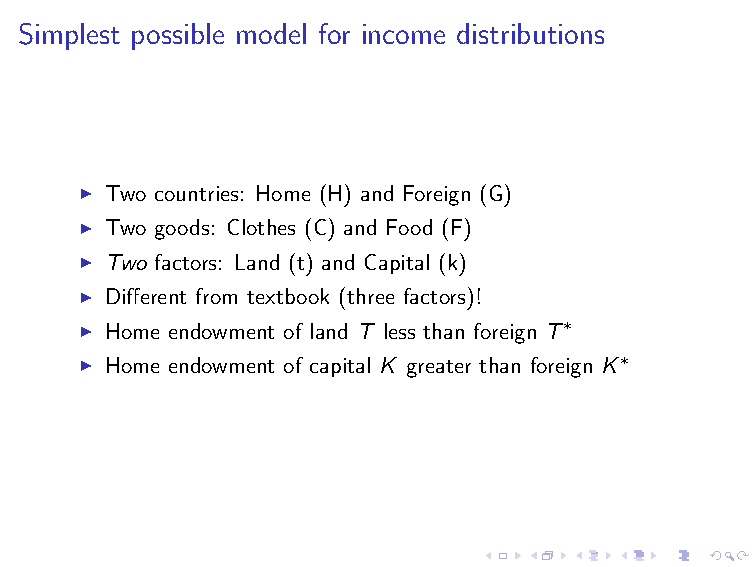
\includegraphics[page=1,width=\textwidth]{review.pdf}}
\frame[plain]{\includegraphics[page=2,width=\textwidth]{review.pdf}}
\frame[plain]{\includegraphics[page=3,width=\textwidth]{review.pdf}}
\frame[plain]{\includegraphics[page=4,width=\textwidth]{review.pdf}}
\frame[plain]{\includegraphics[page=5,width=\textwidth]{review.pdf}}
\frame[plain]{\includegraphics[page=6,width=\textwidth]{review.pdf}}
\frame[plain]{\includegraphics[page=7,width=\textwidth]{review.pdf}}
\frame[plain]{\includegraphics[page=8,width=\textwidth]{review.pdf}}
\frame[plain]{\includegraphics[page=9,width=\textwidth]{review.pdf}}
\frame[plain]{\includegraphics[page=10,width=\textwidth]{review.pdf}}
\frame[plain]{\includegraphics[page=11,width=\textwidth]{review.pdf}}
\frame[plain]{\includegraphics[page=12,width=\textwidth]{review.pdf}}
\frame[plain]{\includegraphics[page=13,width=\textwidth]{review.pdf}}
\frame[plain]{\includegraphics[page=14,width=\textwidth]{review.pdf}}
\frame[plain]{\includegraphics[page=15,width=\textwidth]{review.pdf}}

\begin{frame}
    \begin{itemize}
        \item End review 
    \end{itemize}
\end{frame}

\begin{frame}
\begin{itemize}
    \item Quick note on this Chapter 5 of the textbook.
\end{itemize}

\end{frame}
\begin{frame}{Heckscher-Ohlin: Rise of a theory}

    \begin{itemize}
        \item From a book by Ohlin published in 1933 
        \item Original point $\rightarrow$ trade and long-run income distribution
        \item Attractive model
        \begin{itemize}
            \item Elegant: Can be analyzed graphically
            \item Enough complexity to tackle many trade issues
            \begin{itemize}
                \item Effect of trade liberalization
                \item Effect of tariffs
                \item Effect of technological change on trade patterns
                \item Effect of technological change on income distributions 
            \end{itemize}
            \item Clear, testable predictions
            \item Developed and extended by famous economists
            \begin{itemize}
                \item Ohlin (Nobel 1979)
                \item Samuelson (Nobel 1970)
            \end{itemize}
        \end{itemize}
    \end{itemize}

\end{frame}

\begin{frame}{Heckscher-Ohlin: Downfall}

    \begin{itemize}
        \item Some quotes: 
            \begin{itemize}
                \item \textcolor{blue}{\dots \emph{the Heckscher-Ohlin model is hopelessly inadequate as an explanation for historical and modern trade patterns, unless we allow for technological differences across countries.} }

-Robert Feenstra, Distinguished Professor of Economics at University of California, Davis, 2004
                \item \textcolor{blue}{\emph{It is time to declare Stolper-Samuelson [an important result of the HO model] dead. Stolper-Samuelson says that trade liberalization will raise the real income of the abundant (unskilled) labor in poor countries.  Stolper-Samuelson, qua theorem, is not wrong, of course. But if we use it, as we so often have, as if it provides a reliable answer to this question of real human significance, then it is worse than wrong - it is dangerous.} }

-Donald Davis, Professor of Economics at Colombia University and Prachi Mishra, Senior Economist, IMF 2007
            \end{itemize}
            
    \end{itemize}

\end{frame}

\begin{frame}{Heckscher-Ohlin: Why the hate?}

    \begin{itemize}
        \item Heckscher-Ohlin is a scientific theory: testable predictions
        \item Predictions have often not been backed up by data
        \item Assumptions also seem unusual in the modern world
    \end{itemize}

\end{frame}

\begin{frame}{The point}

    \begin{itemize}
        \item Hecksher-Ohlin about long-run effects of trade
        \item Embodied in the idea that all factors are costlessly mobile
    \end{itemize}

\end{frame}

\begin{frame}{The point}

    \begin{itemize}
        \item Famous implications are the four theorems (paraphrase):
        \begin{enumerate}
            \item \emph{Heckscher-Ohlin}: \textcolor{blue}{Countries with relatively more of a resource will export goods for which that resource is more useful in production} 

\textcolor{red}{ex}: China exports Labor-intensive manufactured goods
            \item \emph{Rybczynski}: \textcolor{blue}{If country gets more of a resource, then the output of the good that uses that resource intensively will rise while the output of the other good will fall.}
\textcolor{red}{ex}: if Denmark got more labor, it would increase its production of textiles
            \item \emph{Stolper-Samuelson}: \textcolor{blue}{A rise in the price of a final good for which a particular resource is more useful in production will increase the payments to that resource}

\textcolor{red}{ex}: if the price of textiles goes up, Chinese workers get higher wages
            \item \emph{Factor-price equalization}: \textcolor{blue}{Trade should cause resource prices to converge}

\textcolor{red}{ex}: Danish and Chinese workers should be paid the same wages
        \end{enumerate}
    \end{itemize}

\end{frame}

\begin{frame}{Model - Plan of attack}

        \begin{itemize}
            \item Setup and assumptions
            \item Production possibilities
            \item Production and prices
            \item Autarchy equilibrium
            \item Trade equilibrium
        \end{itemize}

\end{frame}

\begin{frame}{Setup}

        \begin{itemize}
            \item Two countries: Home (H) and Foreign (G)
            \item Two goods: Clothes (C) and Food (F)
            \item Two factors: Labor (L) and Capital (K)
            \item Sometimes called the 2 x 2 x 2 model
        \end{itemize}

\end{frame}

\begin{frame}{Setup}

        \begin{itemize}
            \item Some terminology
            \begin{itemize}
                \item If $\frac{L}{K} < \frac{L^*}{K^*}$, then Capital is \emph{abundant} in Home, and Labor is \emph{scarce}
                \item If for \emph{any} factor prices, relatively more Labor is used to make Clothes than Food, Clothes are \emph{Labor-intensive}, and Food is \emph{Capital-intensive}
            \end{itemize}
        \end{itemize}
    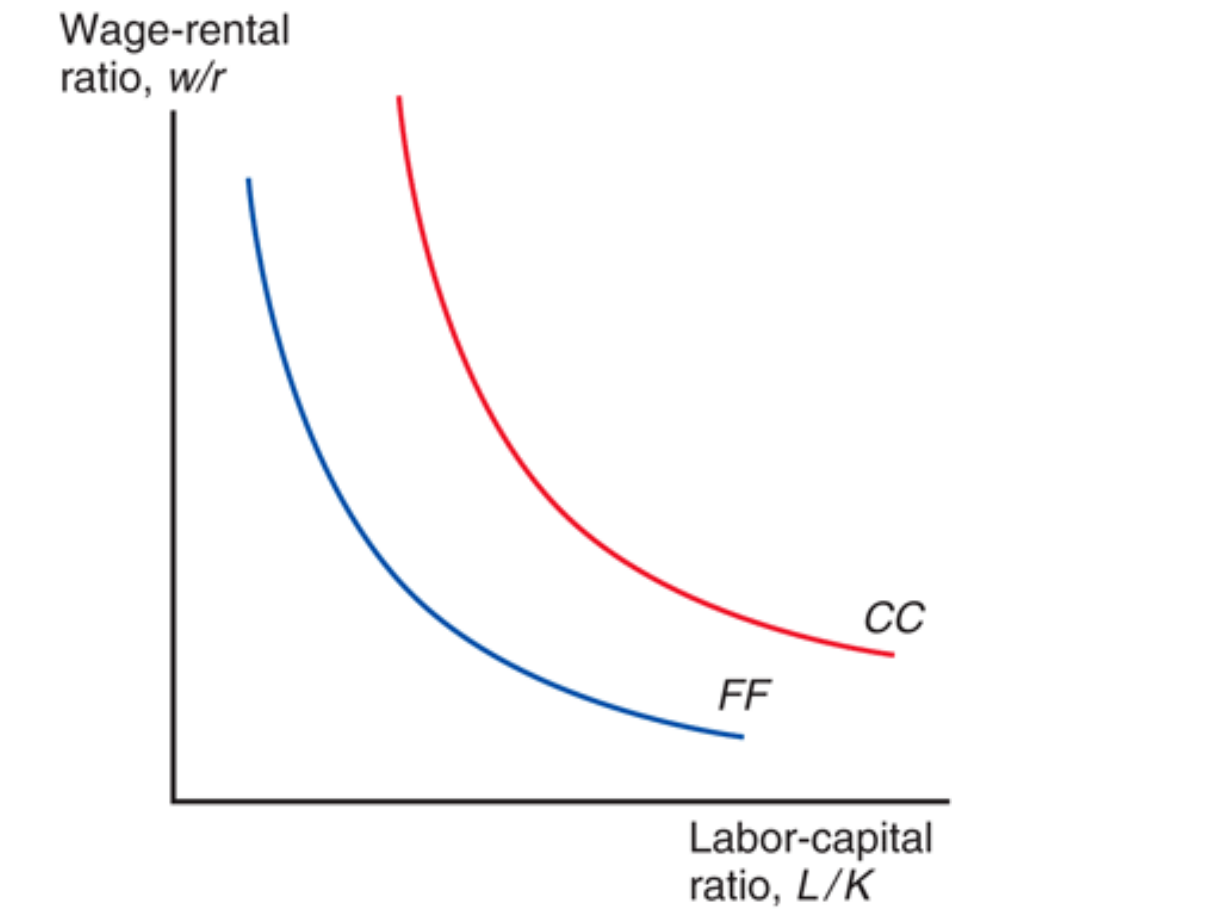
\includegraphics[scale=0.18]{relative_input_prices.png}

\end{frame}

\begin{frame}{Setup}

        \begin{itemize}
            \item Clothes and Food can be produced with combinations of Labor and Capital
            \item Both countries have the same production technology 
            \item Production technologies are Constant Returns to Scale (double both inputs, double output)
            \item Each country has a different endowment of Labor and Capital 
            \item Labor and Capital cannot move between countries, even in the long run
            \begin{itemize}
                \item No shipping of machines allowed
                \item No moving abroad
            \end{itemize}
            \item As before, competitive firms with zero profit
        \end{itemize}

\end{frame}

\begin{frame}{Production Possiblities Frontier}

    \begin{itemize}
        \item Recall:   Slope = take a bit of Labor from Food production and put it into Clothes production
        \item Now also: Slope = take a bit of Capital from Food production and put it into Clothes production
        \item In notation: Slope = $-\frac{MPL_F}{MPL_C} = -\frac{MPK_F}{MPK_C}$ (why must ratios equal?)
    \end{itemize}
    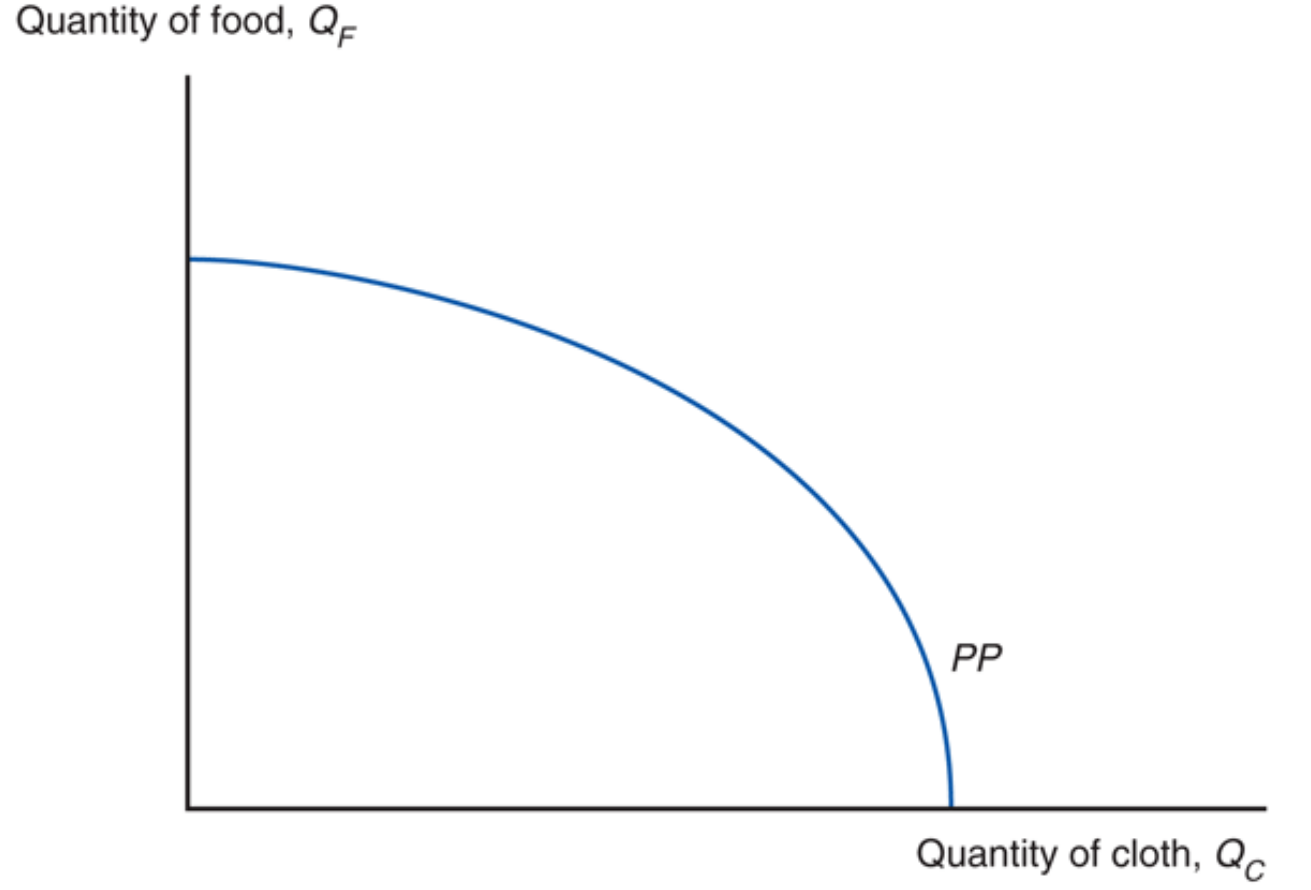
\includegraphics[scale=0.15]{ppf.png}

\end{frame}

\begin{frame}{Input Possiblities}

    \begin{itemize}
        \item Fix the amount of, say, Food we want to produce 
        \item Slope = if I want to use a bit more Labor, how much Capital is freed up? 
        \item $\frac{dQ}{dK} = MPK_F$, $\frac{dK}{dQ} = \frac{1}{MPK_F}$
        \item Slope = $-\frac{\frac{1}{MPK_F}}{\frac{1}{MPL_F}} = -\frac{MPL_F}{MPK_F}$ 
        \item Why is the curve convex?
    \end{itemize}
    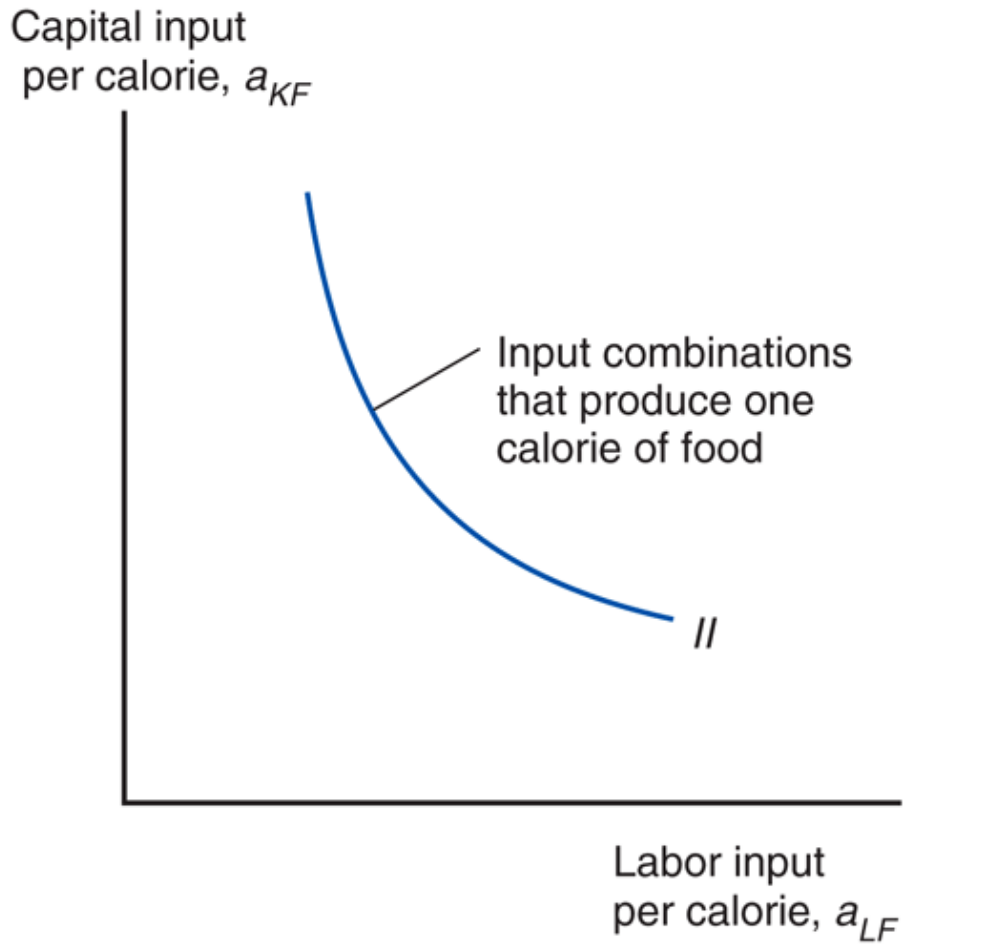
\includegraphics[scale=0.15]{input_poss.png}

\end{frame}

\begin{frame}{Pause}

    \begin{itemize}
        \item We have described the environment
        \item We have described what it is possible to produce
        \item Now how do output prices affect production?
        \item How do input prices affect input choice?
    \end{itemize}

\end{frame}

\begin{frame}{Output price ratio and production}

    \begin{itemize}
        \item Suppose we have the price ratio $\frac{P_C}{P_F}$
        \item Then $\frac{P_C}{P_F} = \frac{MPL_F}{MPL_C} = \frac{MPK_F}{MPK_C}$ (why?)
        \item Production given by the point on the PPF tangent to $-\frac{P_C}{P_F}$
    \end{itemize}
    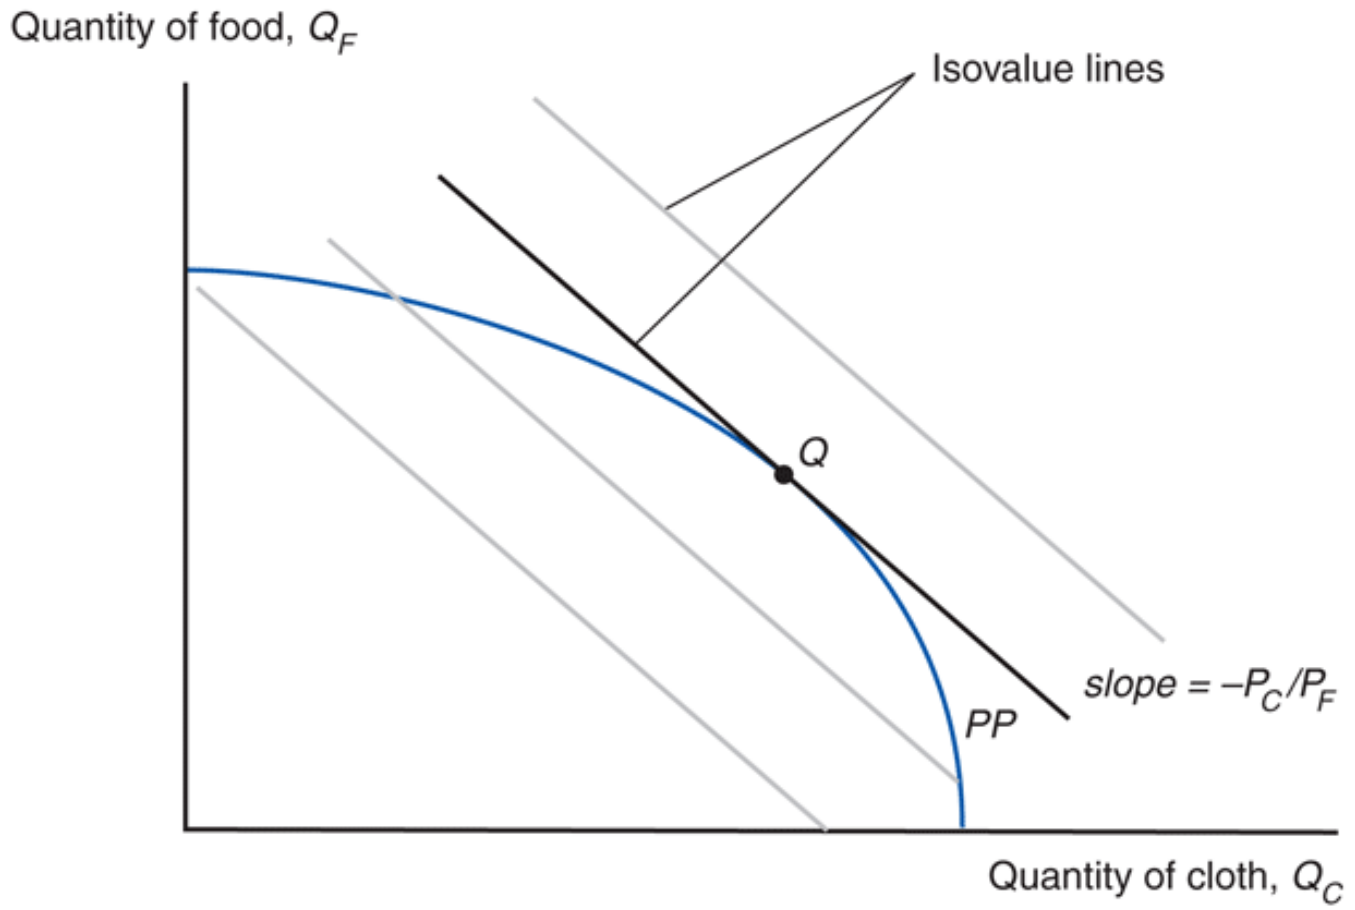
\includegraphics[scale=0.15]{ppf_equil.png}

\end{frame}

\begin{frame}{Input price ratio and production} 
    \begin{itemize}
        \item Suppose we have the price ratio $\frac{w}{r}$
        \item Then $\frac{w}{r} = \frac{MPL_F}{MPK_F} = \frac{MPL_C}{MPK_C}$ (why?)
        \item Input bundle given by the point on the input possibilities curve tangent to $-\frac{w}{r}$
    \end{itemize}
    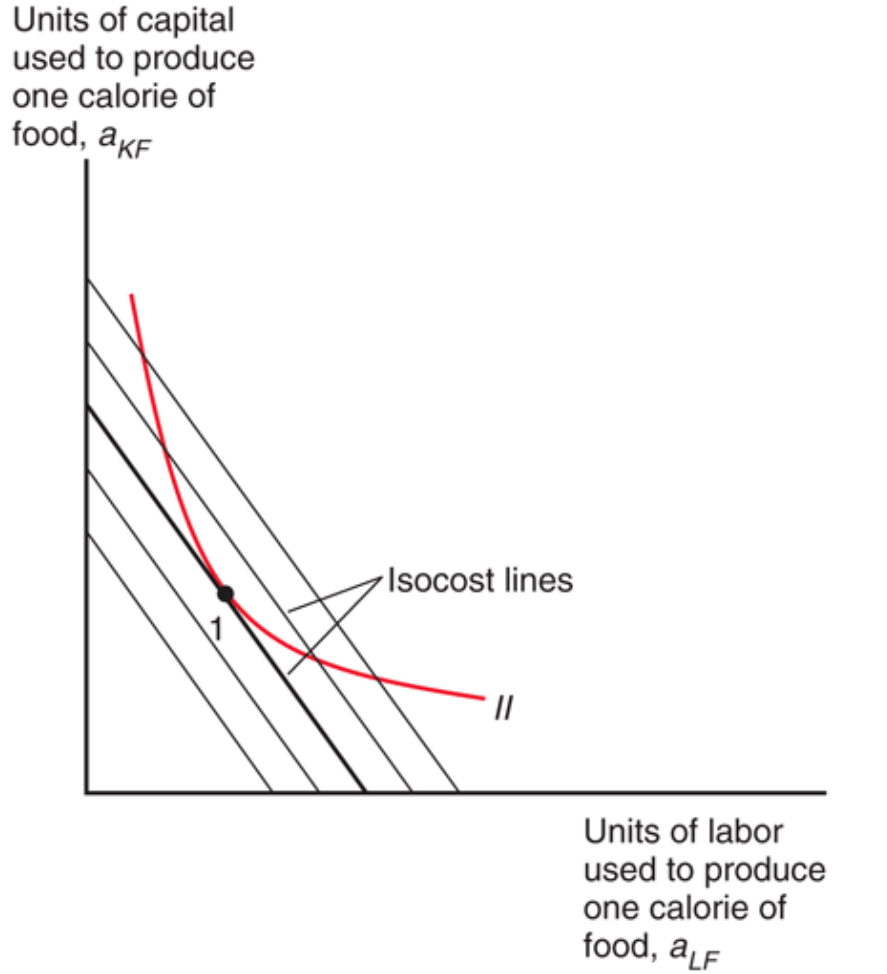
\includegraphics[scale=0.15]{input_cost.png}

\end{frame}

\begin{frame}{Input price change and production}

    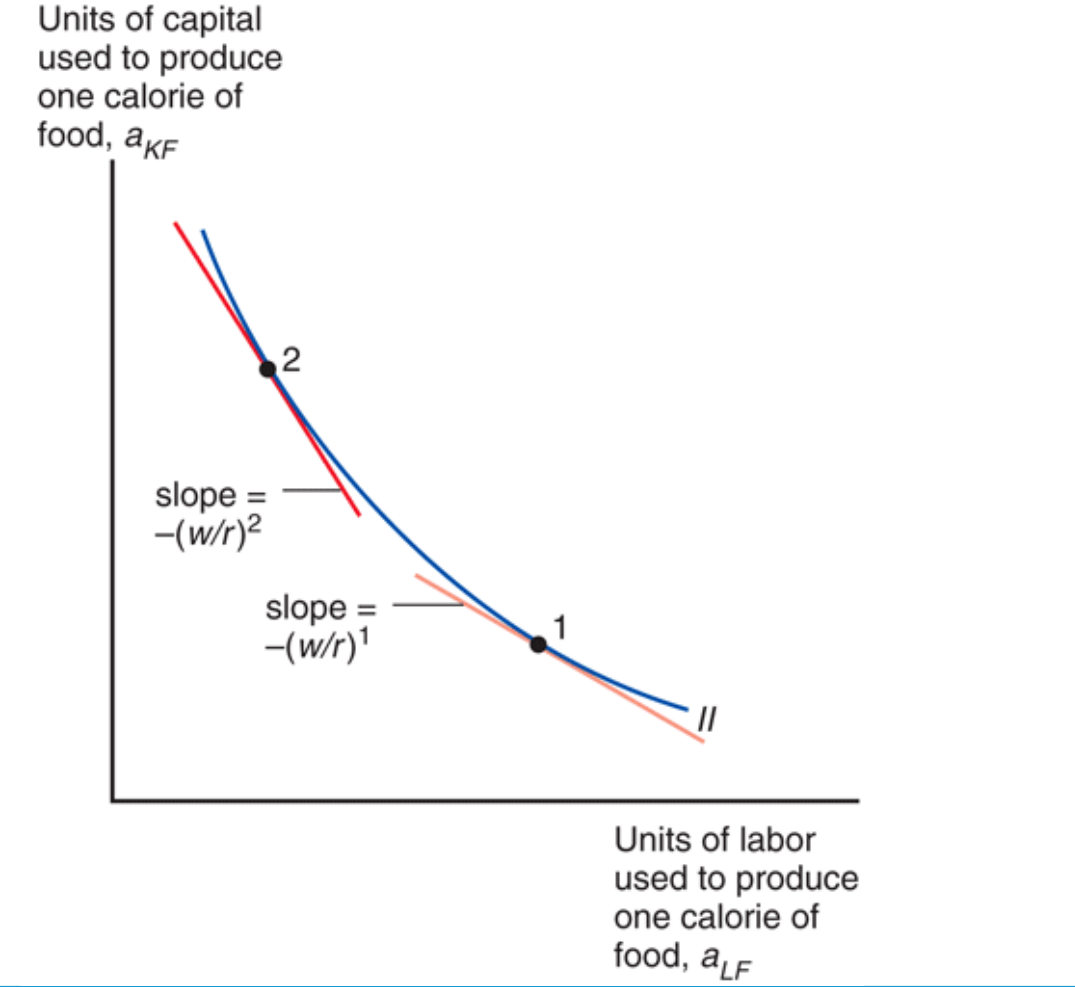
\includegraphics[scale=0.25]{factor_price_change.png}

\end{frame}

\begin{frame}{Pause}

    \begin{itemize}
        \item We have now described what \emph{can} be produced
        \item We have also described how output production is linked to output prices
        \item We have also described how input choice is linked to input prices
        \item Next we will heuristically describe how input and output prices are linked in equilbrium
    \end{itemize}

\end{frame}

\begin{frame}{Input and Output Prices}

    \begin{itemize}
        \item Setup
        \begin{itemize}
            \item Draw input possibilities curves for both goods on the same chart 
            \item Curves are for production of the same value of the two goods 
            \item Assume that both goods are produced
            \item Must be line tangent to both curves, with slope wage-rental ratio
        \end{itemize}
        \item Food industry is \emph{labor intensive}
            \begin{itemize}
        \item That is, for any wage-rental ratio, Food uses a higher proportion of Labor than Clothes
            \end{itemize}
        \item Suddenly the price of food rises
        \begin{itemize}
            \item If wage-rental ratio doesn't change, negative profits for making clothes, clothes industry closes
            \item If both industries to remain open, wage-rental ratio must rise
            \item Since firms hire less labor and more capital per unit produced, $MPL$ rises and $MPK$ falls
            \begin{itemize}
                \item Wages rise (clothes buy more food, and wages paid in clothes rise): $\frac{w}{P_C} = MPL_C = \frac{P_F}{P_C} MPL_F$.  
                \item rent falls (food buys less clothes, and rent paid in food falls): $\frac{r}{P_F} = \frac{P_C}{P_F} MPK_C = MPK_F$.  
            \end{itemize}
        \end{itemize}

    \end{itemize}

\end{frame}

\begin{frame}{The Stolper-Samuelson Theorem}

    \begin{itemize}
            \item \emph{Stolper-Samuelson}: \textcolor{blue}{A rise in the price of a final good for which a particular resource is more useful in production will increase the payments to that resource}
            \item Owners of one input are always hurt by a price change in output goods.
            \item Trade in outputs typically changes output prices, so some people are typically hurt by trade.
    \end{itemize}

\end{frame}

\begin{frame}{Textbook discussion of Stolper-Samuelson}

    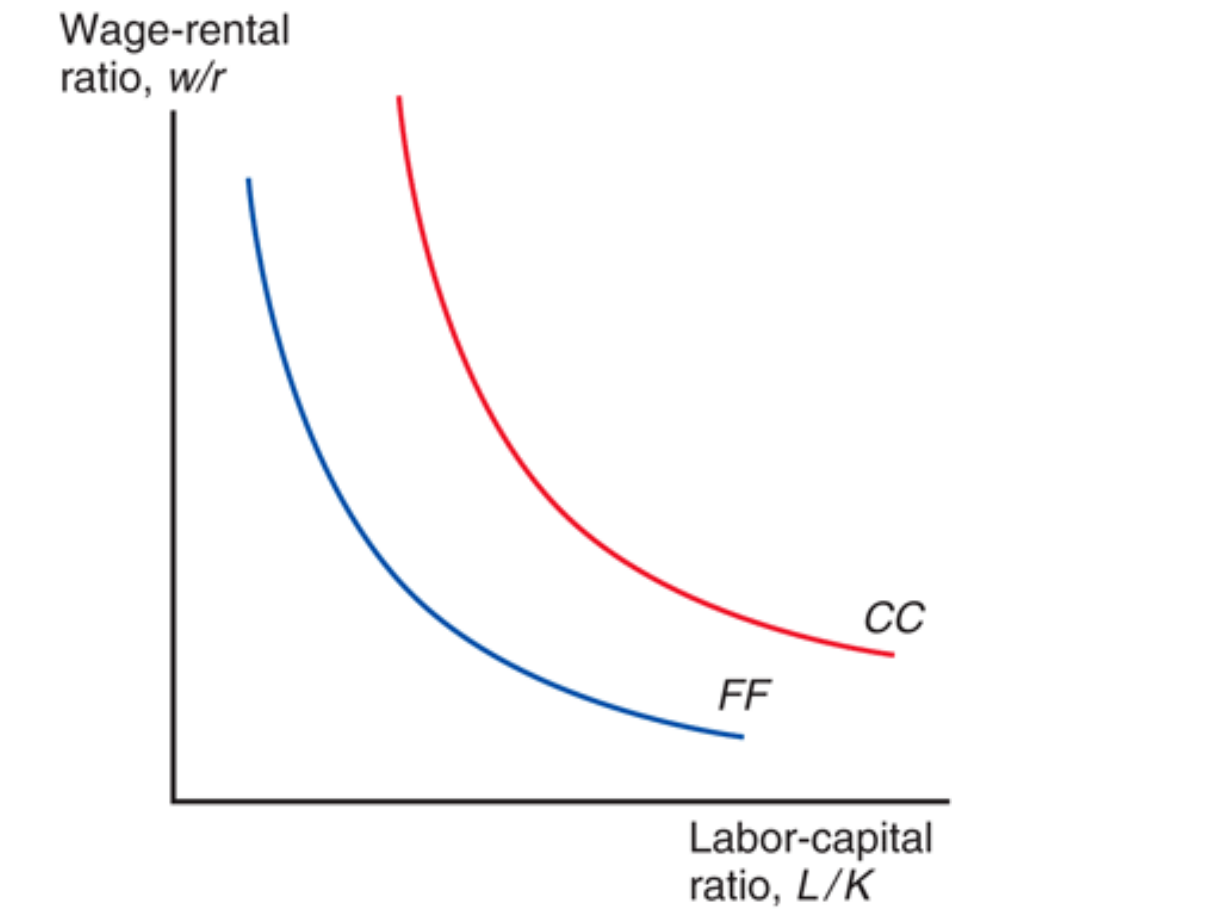
\includegraphics[scale=0.2]{relative_input_prices.png}

\end{frame}

\begin{frame}{Textbook discussion of Stolper-Samuelson}

    \begin{itemize}
        \item Heuristic: Clothes use relatively more labor, so if price of labor relatively increases, $\frac{P_C}{P_F}$ increases.
        \item How did we derive this relationship?
    \end{itemize}
    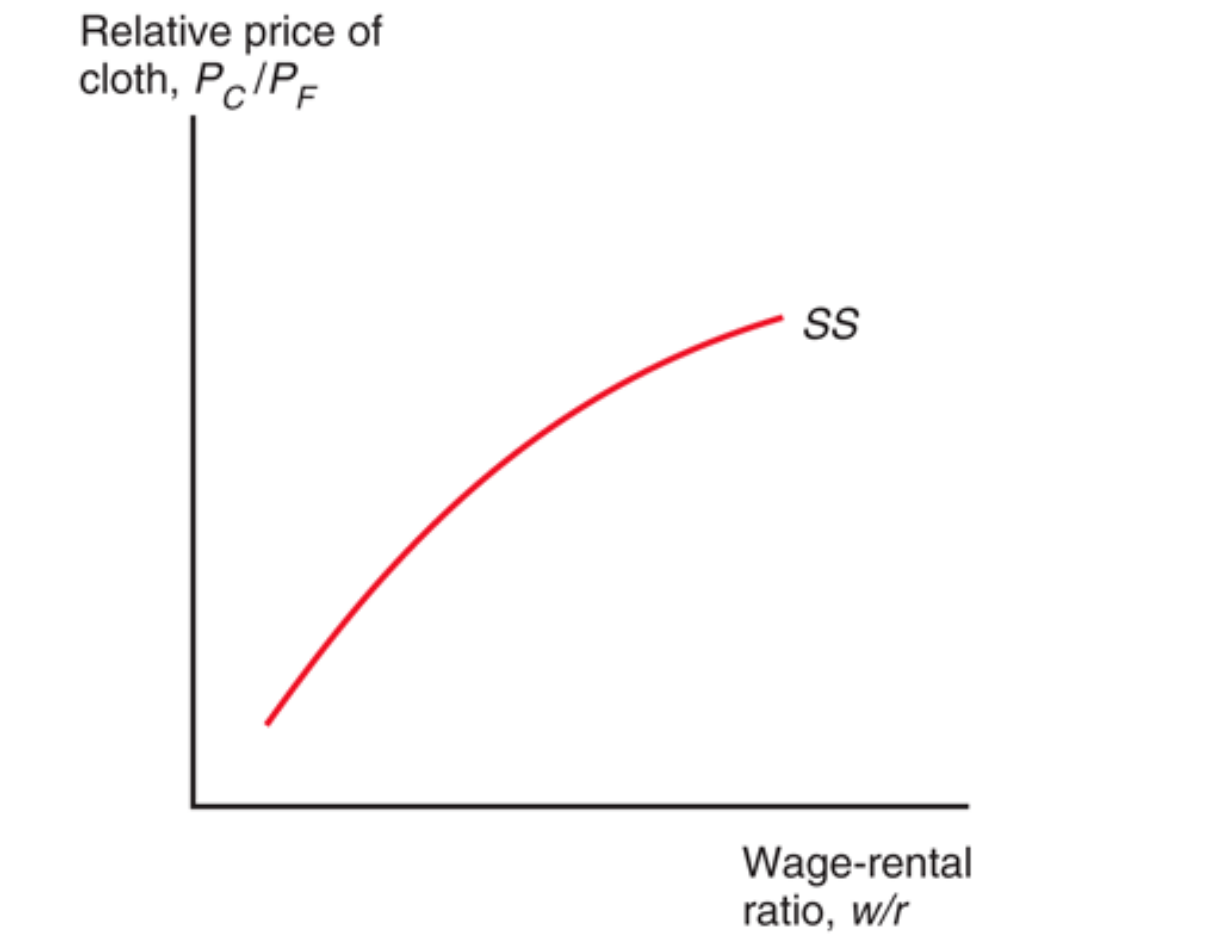
\includegraphics[scale=0.2]{rel_price_input_price.png}

\end{frame}

\begin{frame}{Textbook discussion of Stolper-Samuelson}

    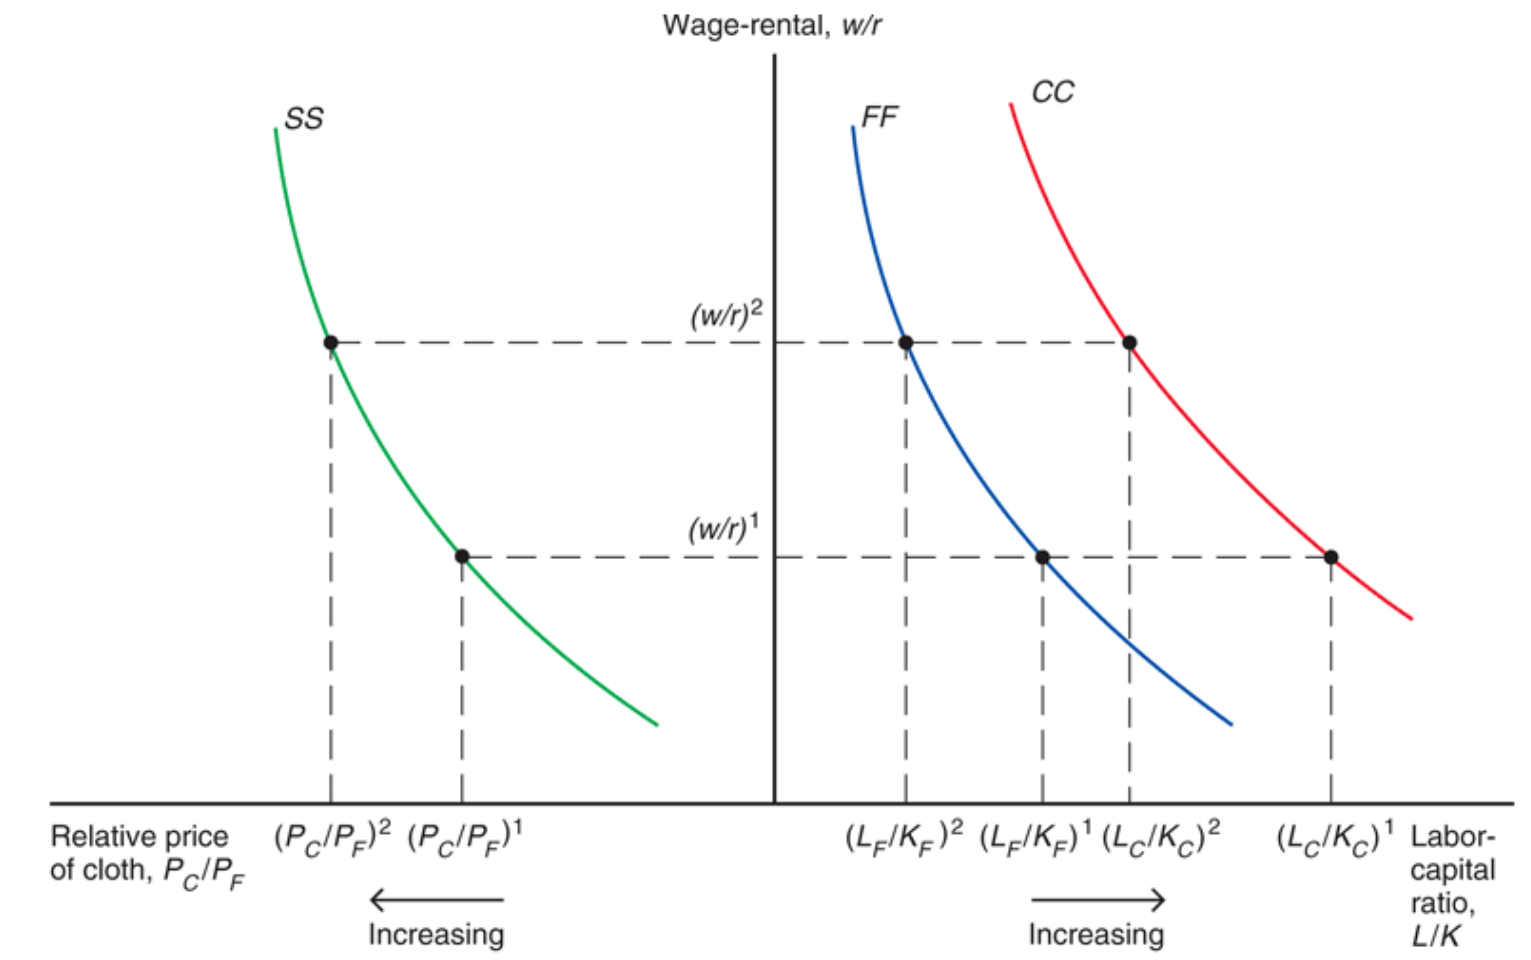
\includegraphics[scale=0.2]{sidebyside.png}

\end{frame}

\begin{frame}{Pause} 
    \begin{itemize}
        \item We have now described what \emph{can} be produced
        \item We have described how output production is linked to output prices
        \item We have described how input choice is linked to input prices
        \item We have described how input and output prices are linked (Stolper-Samuelson)
        \item Next: Fixing prices, how do changes in factor endowments affect production?
    \end{itemize}

\end{frame}

\begin{frame}{Factor endowment changes and production}

    \begin{itemize}
        \item If prices do not change, industry-level Labor-Capital ratios do not depend on aggregate Labor-Capital ratios 
    \end{itemize}
    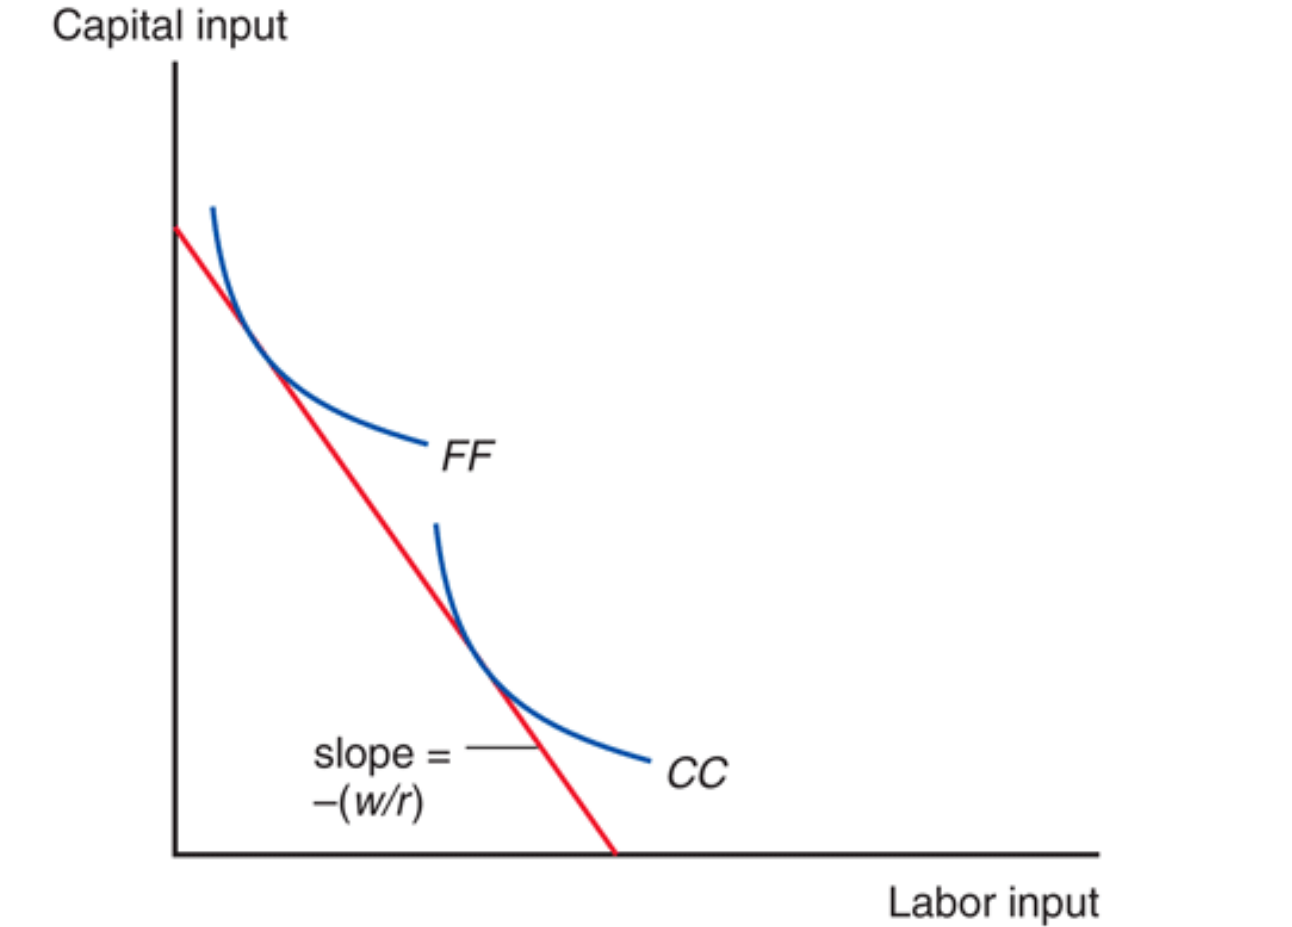
\includegraphics[scale=0.2]{two_factor_choice.png}

\end{frame}

\begin{frame}{Factor endowment changes and production}

    \begin{itemize}
        \item We have the accounting identity:
        \begin{align*}
            \frac{L}{K} &= \frac{L_C}{K} + \frac{L_F}{K} \\
            &= \frac{L_C}{K_C}\frac{K_C}{K} + \frac{L_F}{K_F} \frac{K_F}{K}
        \end{align*}
        \item Changes in aggregate $\frac{L}{K}$ do not affect $\frac{L_C}{K_C}$ and $\frac{L_F}{K_F}$
        \item If $\frac{L}{K}$ increases, only way for the identity to hold is for Capital to move from the capital intensive industry to the labor intensive industry
        \item If Capital moves, since industry Capital-Labor ratios don't change, Labor must move as well
        \item That is, $\frac{L}{K}$ increases $\rightarrow$ more Labor-intensive good, less Capital-intensive good
    \end{itemize}

\end{frame}

\begin{frame}{The Rybczynski Theorem}
    \begin{itemize}
            \item \emph{Rybczynski}: \textcolor{blue}{If country gets more of a factor, then the output of the good that uses that factor intensively will rise while the output of the other good will fall.}
    \end{itemize}
\end{frame}

\begin{frame}{Pause}

    \begin{itemize}
        \item We have now described what \emph{can} be produced
        \item We have described how production and inputs linked to prices
        \item We have described how input and output prices are linked (Stolper-Samuelson)
        \item We have described how factor endowments and output is linked (Rybczynski) 
        \item Next: Describe trade patterns in equilibrium
    \end{itemize}

\end{frame}

\begin{frame}{Trade Patterns}

    \begin{itemize}
        \item Remember: Countries are identical, except for relative factor endowments 
        \item Assume that home has relatively more Capital: $\frac{L}{K} < \frac{L^*}{K^*}$
        \item For \emph{any} output price, Rybczynski $\rightarrow$ relatively more Capital intensive good (Clothing) produced at home:
            \begin{equation*}
                \frac{Q_C}{Q_F} > \frac{Q_C^*}{Q_F^*}
            \end{equation*}
        \item Since consumption depends only on output price, equilibrium consumption ratio $\frac{D_C}{D_F} = \frac{D_C^*}{D_F^*}$
        \item (Hidden assumption: homotheticity again!)
        \item Must be that home exports Capital-intensive good (Clothes) and imports Labor-intensive good (Food)
    \end{itemize}

\end{frame}
            
\begin{frame}{The Hecksher-Ohlin Theorem}

    \begin{itemize}
            \item The country with relatively more Capital exports the Capital-intensive good.
            \item The country with relatively more Labor exports the Labor-intensive good.
            \item \emph{Heckscher-Ohlin}: \textcolor{blue}{Countries with relatively more of a resource will export goods for which that resource is more useful in production}
    \end{itemize}
\end{frame}

\begin{frame}{The effect of trade on relative input and output prices}

    \begin{itemize}
            \item Claim in the book: Trade induces convergence in relative output prices
            \item Notice that relative price change in favor of abundent resource in both countries
    \end{itemize}
    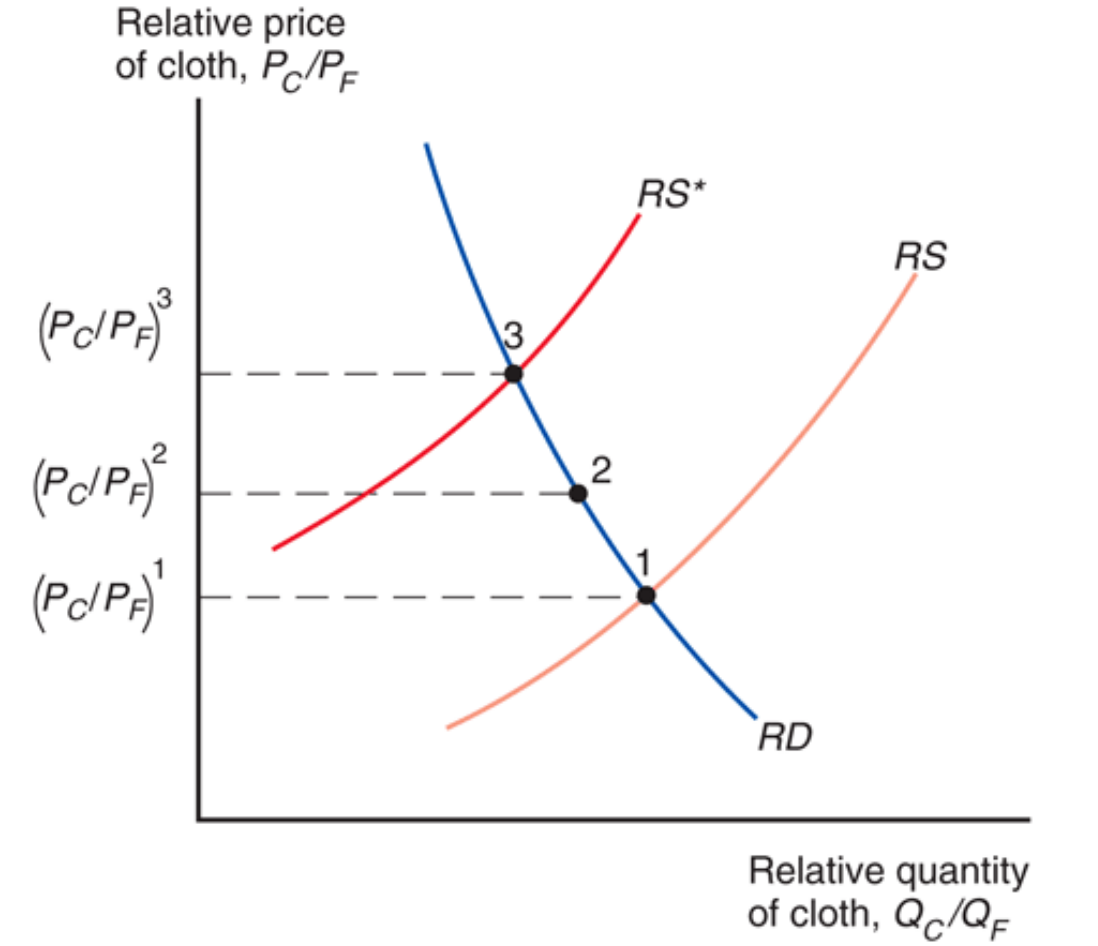
\includegraphics[scale=0.2]{trade_price_convergence.png}
\end{frame}

\begin{frame}{The effect of trade on relative prices}

    \begin{itemize} 
         \item If this (fairly reasonable) claim is true:
             \begin{itemize}
                \item Owners of the abundent resource gain
                \item Owners of the scarce resource lose
                \item Reason: Stolper-Samuelson theorem
            \end{itemize}
         \item Trade should hurt skilled Chinese labor, and unskilled Danish labor
    \end{itemize}

\end{frame}

\begin{frame}{Pause}

    \begin{itemize}
        \item We have now described what \emph{can} be produced
        \item We have described how production and inputs linked to prices
        \item We have described how input and output prices are linked (Stolper-Samuelson)
        \item We have described how factor endowments and output is linked (Rybczynski) 
        \item We have described trade patterns in equilibrium (Heckscher-Ohlin)
        \item Next, we will describe the effect of trade on factor prices
    \end{itemize}

\end{frame}

\begin{frame}{The effect of trade on world factor prices}

    \begin{itemize} 
         \item In our proof of Stolper-Samuelson, we saw a graph as below showing how factor prices are determined in equilibrium
        \item This graph is related only to the technology available and relative price of the two goods 
        \item This graph is \emph{not} related to aggregate factor endowments $\frac{L}{K}$ and $\frac{L^*}{K^*}$
        \item Since in trade relative prices are the same, and technologies in the countries are the same:
        \begin{itemize}
            \item So are factor prices the same in the two countries!
        \end{itemize}
        \item Intuition: Exporting the Labor-intensive good is like exporting Labor, even though Labor cannot move between countries
     \end{itemize}

\end{frame}

\begin{frame}{The Four Theorems}

    \begin{itemize}
        \item Famous implications are the four theorems:
        \begin{enumerate}
            \item \emph{Heckscher-Ohlin}: \textcolor{blue}{Countries abundent in a factor will export the good intensive in that factor} 
            \item \emph{Rybczynski}: \textcolor{blue}{If a country's relative amount of a factor rises, then the output of the good intensive in that factor will rise while the output of the other good will fall.}
            \item \emph{Stolper-Samuelson}: \textcolor{blue}{A rise in the relative price of an output intensive in a factor will increase thereal returns to that factor, and decrease returns to the other factor}
            \item \emph{Factor-price equalization}: \textcolor{blue}{Trade causes factor prices to completely converge}
        \end{enumerate}
        \item Empirical tests will be based on these four predictions
    \end{itemize}

\end{frame}

\begin{frame}{Problems - assumptions}

    \begin{enumerate}
        \item Proofs of the theorems require that both goods are produced in both countries
        \item The model assumes technology is the same everywhere
        \item The model assumes that Capital cannot move
        \item Output goods have the same price everywhere
    \end{enumerate}
    \begin{itemize}
        \item In the early 20th century, these assumptions were reasonable
        \item Now they seem like a poor approximation to the world
    \end{itemize} 
\end{frame}

\begin{frame}{Factor price equalization}

    \begin{itemize}
        \item Most obvious test
        \item Most obvious failure, even as an approximation
    \end{itemize}
    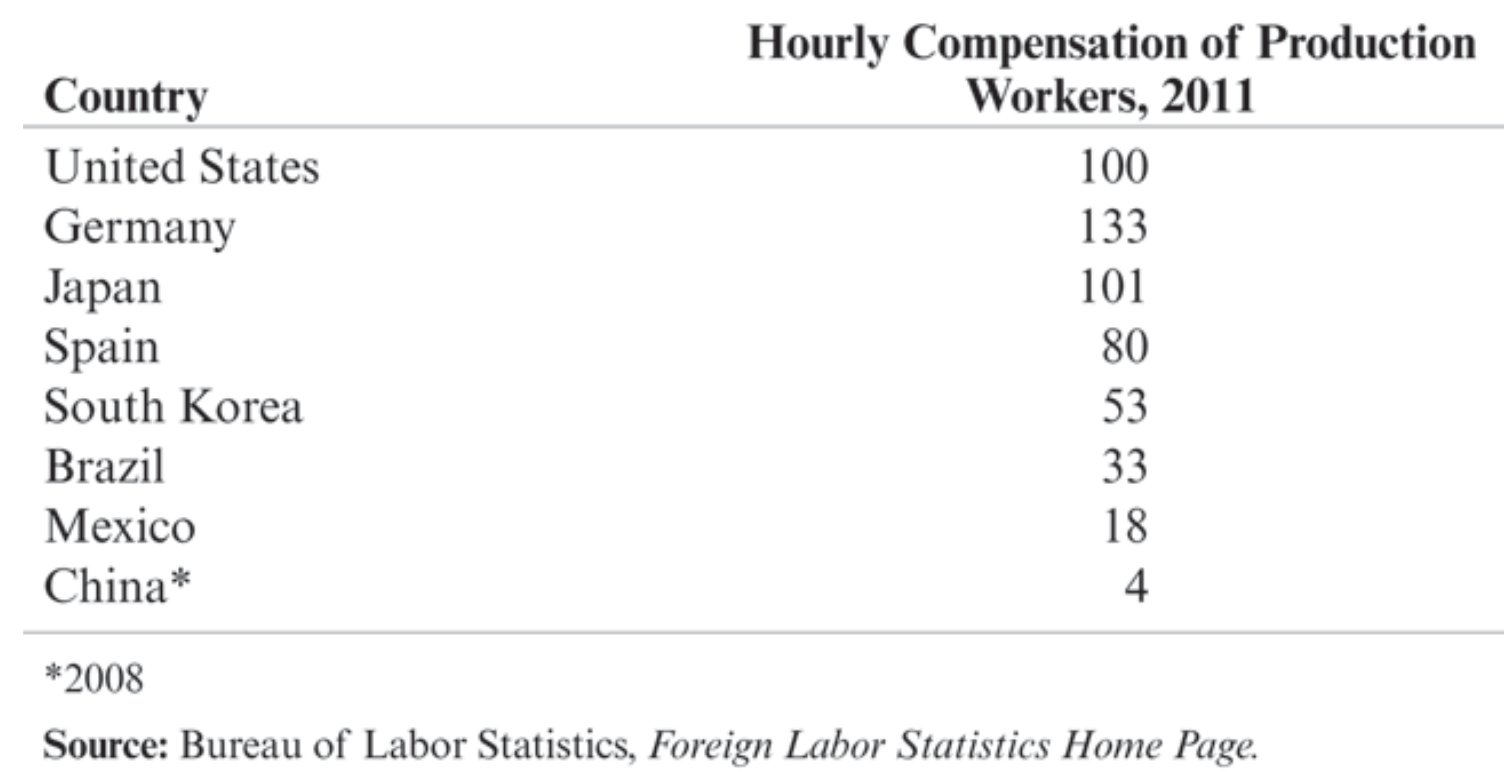
\includegraphics[scale=0.2]{factor_price_differences.png}

\end{frame}

\begin{frame}{Reduction in developing country inequality}

    \begin{itemize}
        \item Suppose our two factors were skilled and unskilled Labor 
        \item China is abundent in unskilled Labor, Denmark in skilled
        \item Trade liberalization should cause China to export goods intensive in unskilled Labor (Heckscher-Ohlin)
        \item This should cause the relative price of goods intensive in unskilled Labor to rise in China
        \item That should increase the returns to unskilled Labor relative to skilled labor (Stolper-Samuelson)
        \item Less wage inequality predicted!
    \end{itemize}

\end{frame}

\begin{frame}{Reduction in devloping country inequality}

    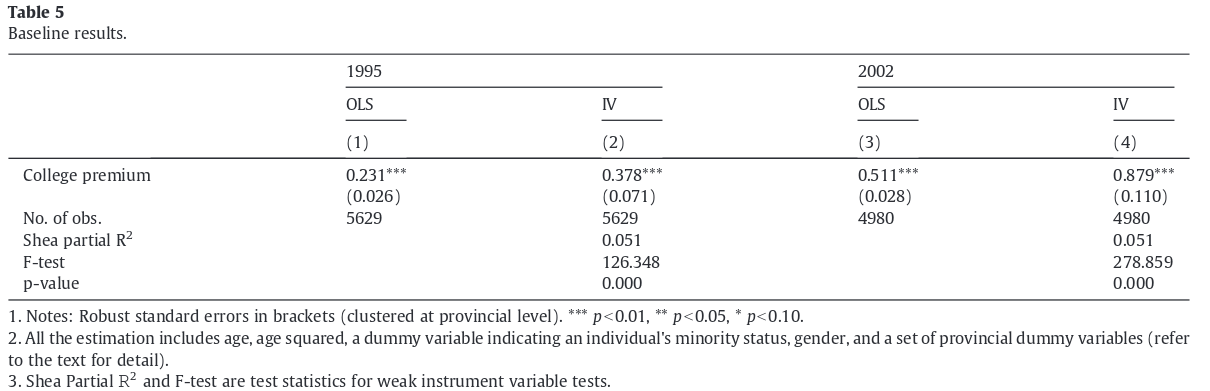
\includegraphics[scale=0.25]{LWang_CER_2012.png}
    {\tiny Source: Wang, L. Economic Transition and College Premium in Urban China, China Economic Review, 2012}

\end{frame}

\begin{frame}{The flip side}

    \begin{itemize}
        \item Of course, we should also expect the college premium to go up in developed countries
    \end{itemize}
    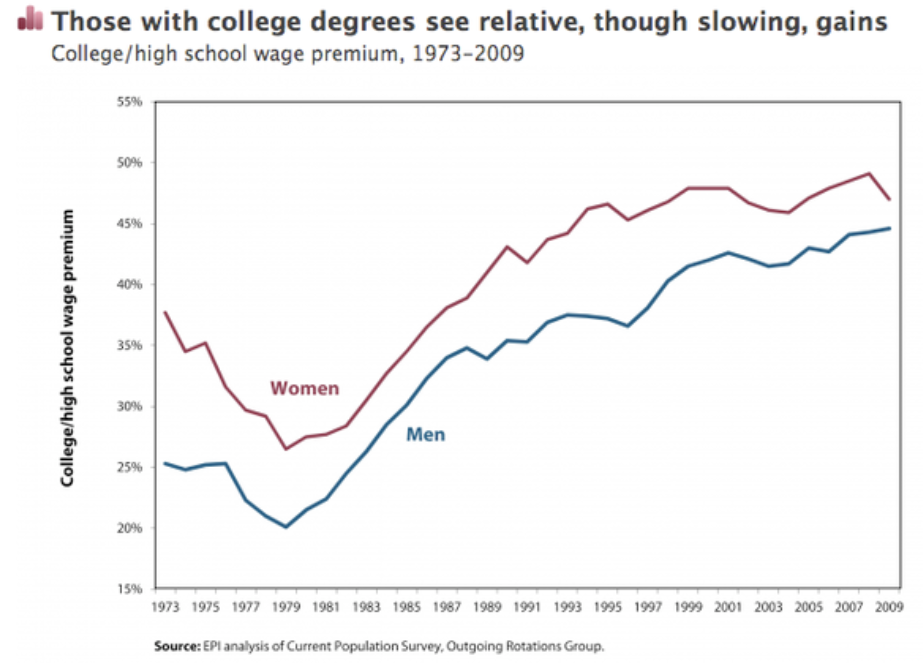
\includegraphics[scale=0.25]{US_college_premium.png}

\end{frame}

\begin{frame}{The Leontief Paradox}

    \begin{itemize}
        \item Heckscher Ohlin Theorem says that the United States should export Capital intensive goods, and import Labor intensive goods
        \item Leontief pointed out that the opposite is true, that is the sign of trade is incorrect
        \item More recently, Davis and Weinstein find that trade patterns fail the HO sign test for 64\% of countries 
        \item The HO predictions are worse than random!
    \end{itemize}

\end{frame}

\begin{frame}{Missing trade}

    \begin{itemize}
        \item The United States and Europe have a very large share of world Capital, but a very small share of world Labor 
        \item The opposite is true for developing countries 
        \item We should see massive trade flows between the developed and developing world
        \item In reality we see very little trade relative to developing developing trade
    \end{itemize}

\end{frame}

\begin{frame}

    \begin{itemize}
        \item If we start dropping assumptions, the HO predictions to better
        \begin{enumerate}
            \item Common technologies across countries 
            \item Countries produce the same set of goods
            \item Costless trade, equalized output prices
        \end{enumerate}
    \end{itemize}

    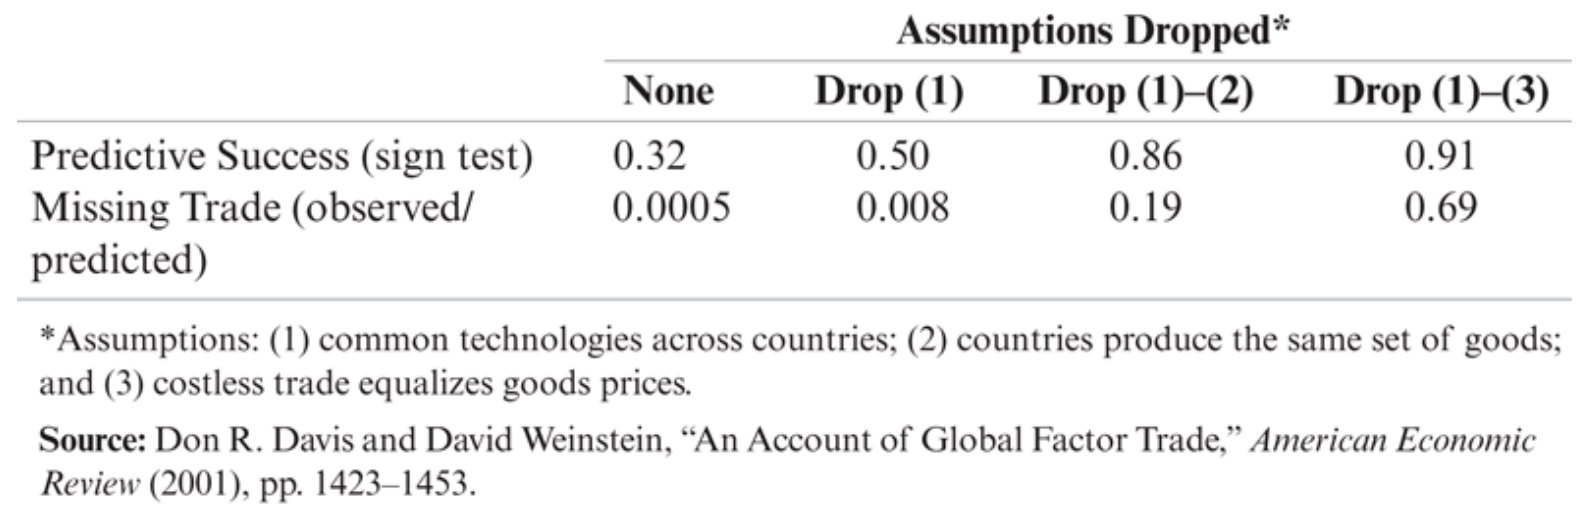
\includegraphics[scale=0.20]{davidweinstein.png}
\end{frame}

\begin{frame}{My view}

    \begin{itemize}
        \item We used these assumptions to prove the theorems
        \item Without the theorems, the model does not have predictions
        \item Therefore, if we drop the assumptions, we do not really have a test
    \end{itemize}

\end{frame}

\begin{frame}{Where the HO model does better}

    \begin{itemize}
        \item Skill intensity in developed and developing country exports
    \end{itemize}
    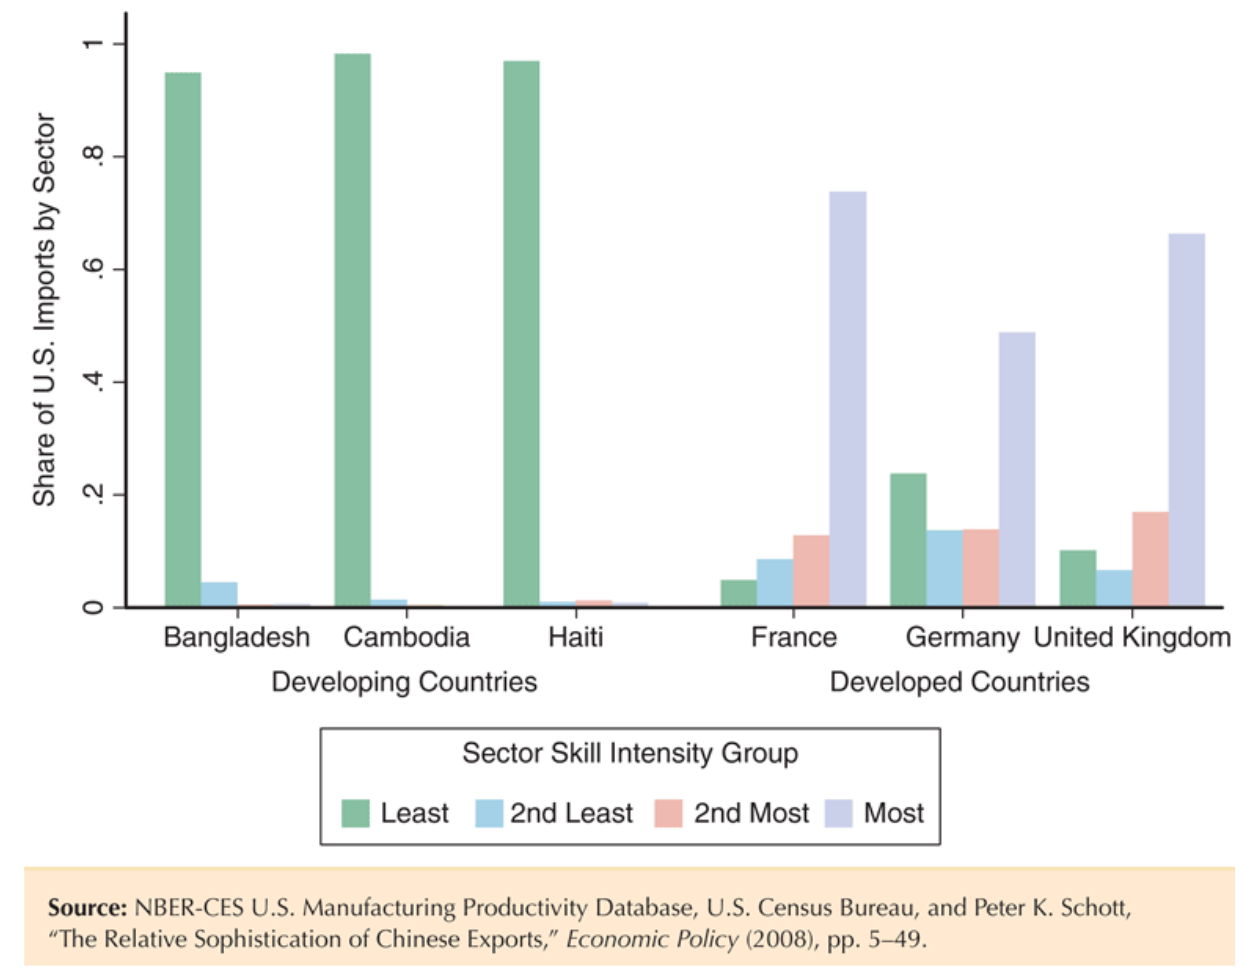
\includegraphics[scale=0.20]{schott1.png}

\end{frame}

\begin{frame}{where the HO model does better}

    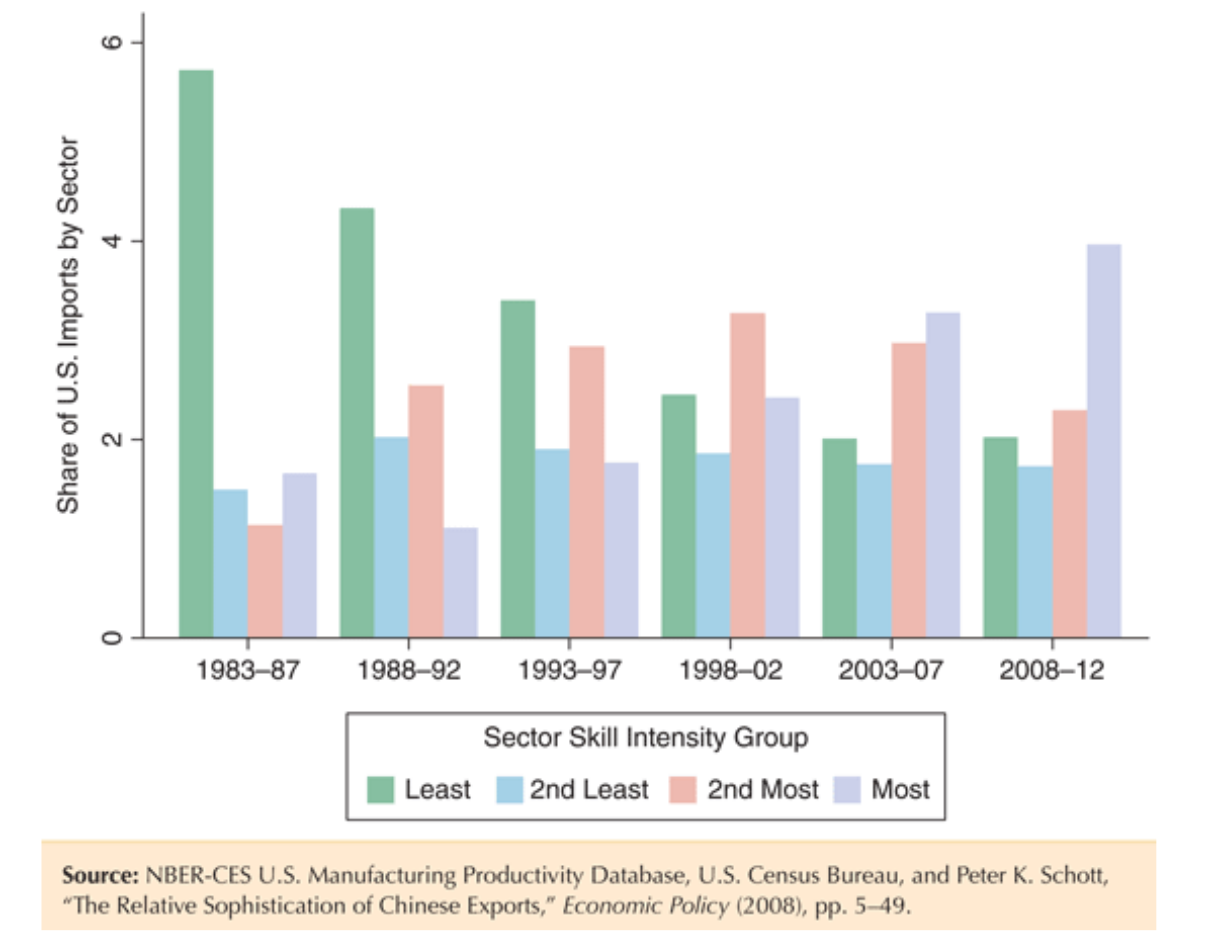
\includegraphics[scale=0.23]{china_schott.png}

\end{frame}

\begin{frame}{where the HO model does better}

    \begin{itemize}
        \item Then again, hard to imagine a world were Haiti exports microprocessors and Denmark buttons.
    \end{itemize}

\end{frame}

\begin{frame}{Summary}
        
        \begin{itemize}
            \item Heckscher-Ohlin Theory exteremly important in the history of economic thought on trade
            \item Point: Trade has long-run effects on the distribution of income
            \item Main predictions relate to the four theorems 
            \begin{enumerate}
                \item Heckscher-Ohlin
                \item Rybczynski
                \item Stolper-Samuelson
                \item Factor Price Equalization
            \end{enumerate}
            \item In the last 20 years, theory has become less popular as it has failed to match trade data, even as an approximation
        \end{itemize}

\end{frame}

\begin{frame}{Moving forward}
        
        \begin{itemize}
            \item Next time: ``The Standard Trade Model''
            \item We have seen that HO does better when combined with technology differences
            \item Unifying trade framework with elements from Ricardo, specific factors, and HO. 
            \item Use this model to analyze effect of tariffs, changes in exchange rates, etc
        \end{itemize}

\end{frame}

\frame[plain]{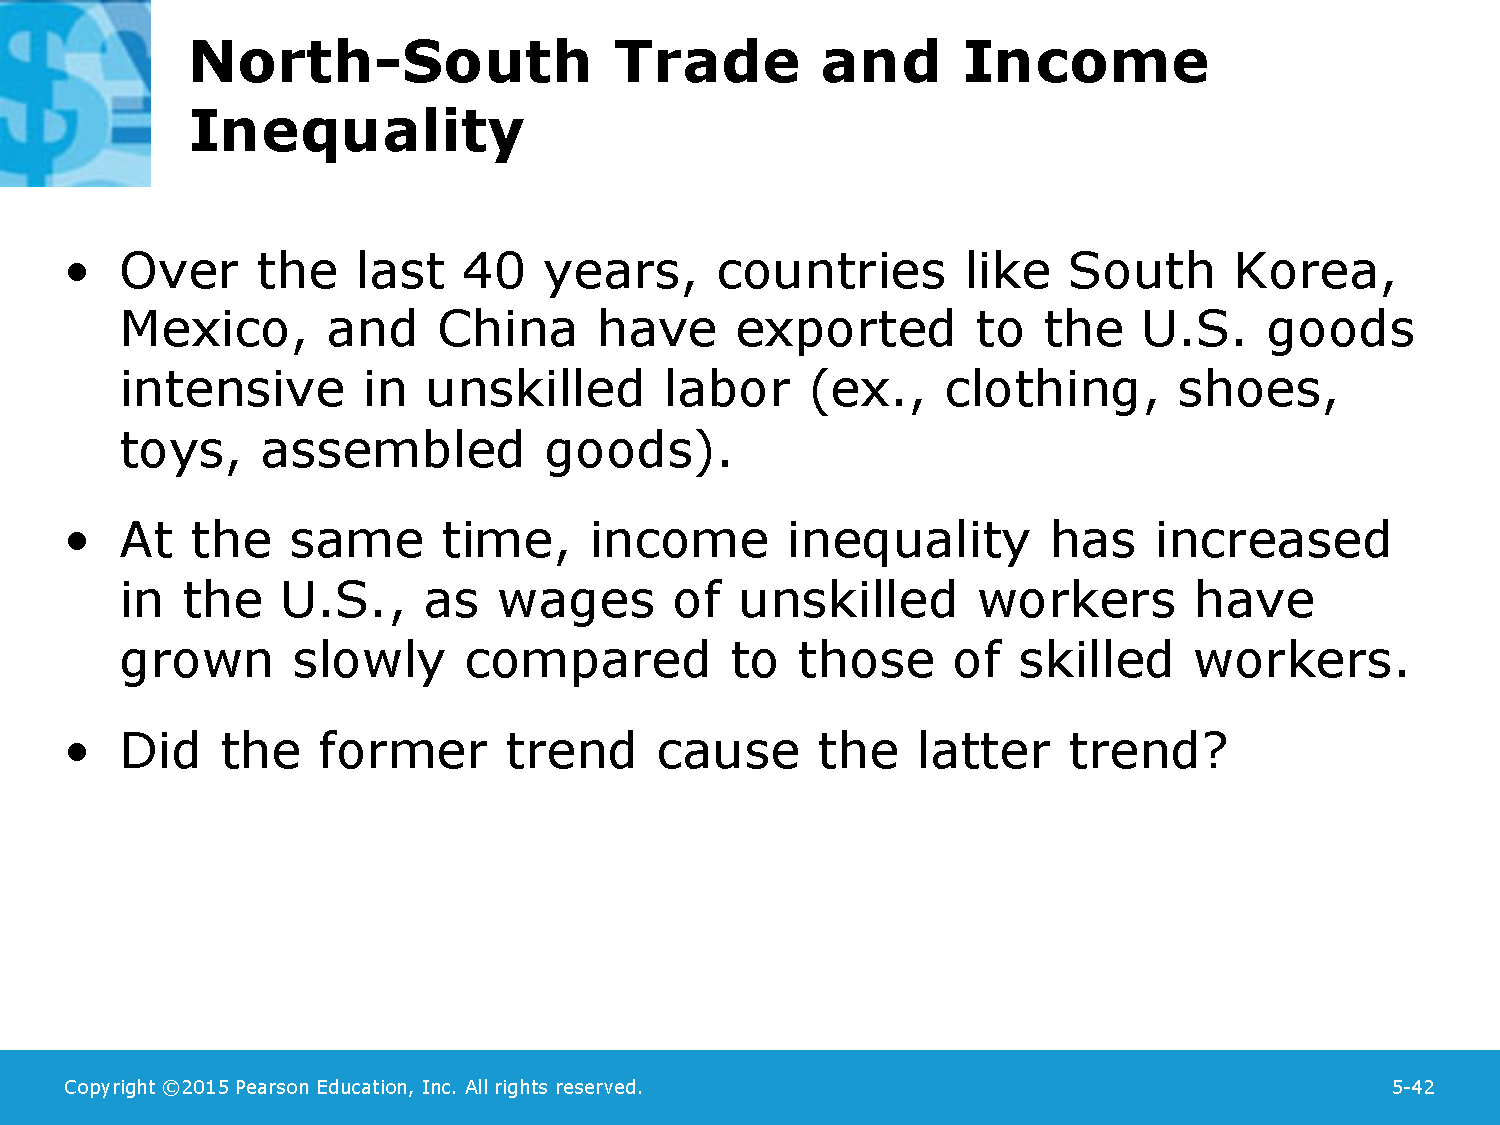
\includegraphics[page=1,width=\textwidth]{Session_4_Heckscher_Ohlin_Pearson_appendix.pdf}}
\frame[plain]{\includegraphics[page=2,width=\textwidth]{Session_4_Heckscher_Ohlin_Pearson_appendix.pdf}}
\frame[plain]{\includegraphics[page=3,width=\textwidth]{Session_4_Heckscher_Ohlin_Pearson_appendix.pdf}}
\frame[plain]{\includegraphics[page=4,width=\textwidth]{Session_4_Heckscher_Ohlin_Pearson_appendix.pdf}}
\frame[plain]{\includegraphics[page=5,width=\textwidth]{Session_4_Heckscher_Ohlin_Pearson_appendix.pdf}}
\frame[plain]{\includegraphics[page=6,width=\textwidth]{Session_4_Heckscher_Ohlin_Pearson_appendix.pdf}}
\frame[plain]{\includegraphics[page=7,width=\textwidth]{Session_4_Heckscher_Ohlin_Pearson_appendix.pdf}}
\frame[plain]{\includegraphics[page=8,width=\textwidth]{Session_4_Heckscher_Ohlin_Pearson_appendix.pdf}}

\end{document}






